\documentclass[a4paper,10pt]{article}
\usepackage[utf8x]{inputenc}
\usepackage{verbatim}
\usepackage{graphicx}
\usepackage{enumerate}

%opening
\title{Lab 7}
\author{William Richard}

\begin{document}

\maketitle

\section{Cron}
\subsection{Original cronfile, with friday run}
  \begin{center}
  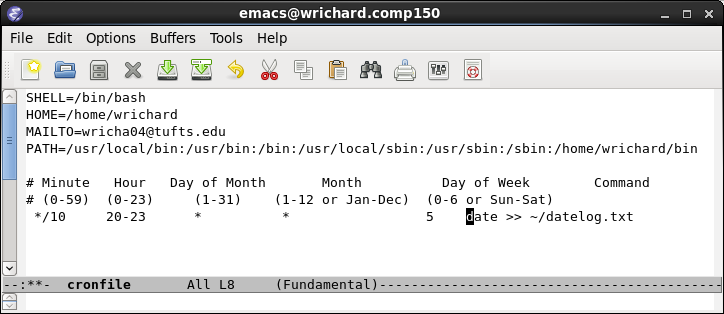
\includegraphics[width=\linewidth]{./fri_cronfile.png}
  \end{center}

\subsection{Installed original cronfile}
  \begin{center}
  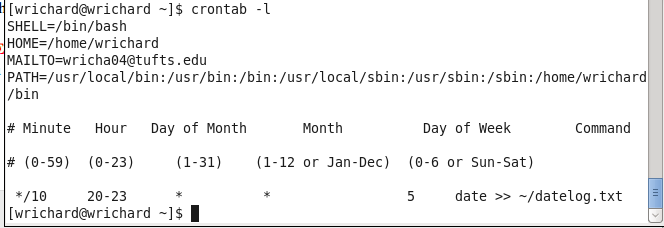
\includegraphics[width=\linewidth]{./crontab_list_fri.png}
  \end{center}

\subsection{Edit to Tuesday run}
  \begin{center}
  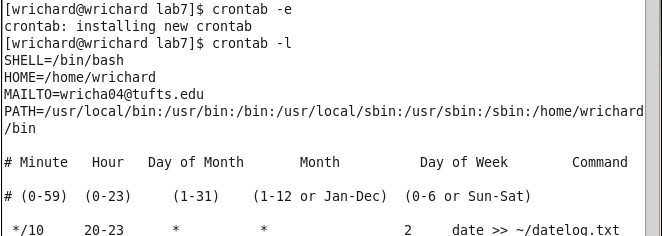
\includegraphics[width=\linewidth]{./crontab_e.png}
  \end{center}

\subsection{Today is Saturday}
Because today is Saturday, I have adjusted my crontab as pictured below to run on Saturdays from 8-12.  This way, I can show you that my file works.

  \begin{center}
  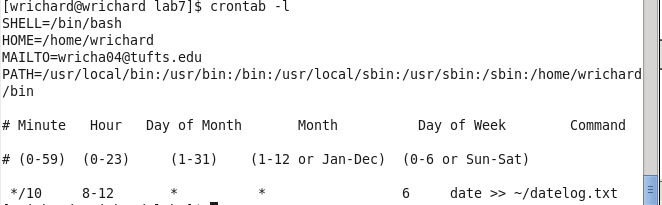
\includegraphics[width=\linewidth]{./crontab_sat.png}
  \end{center}

  \begin{center}
  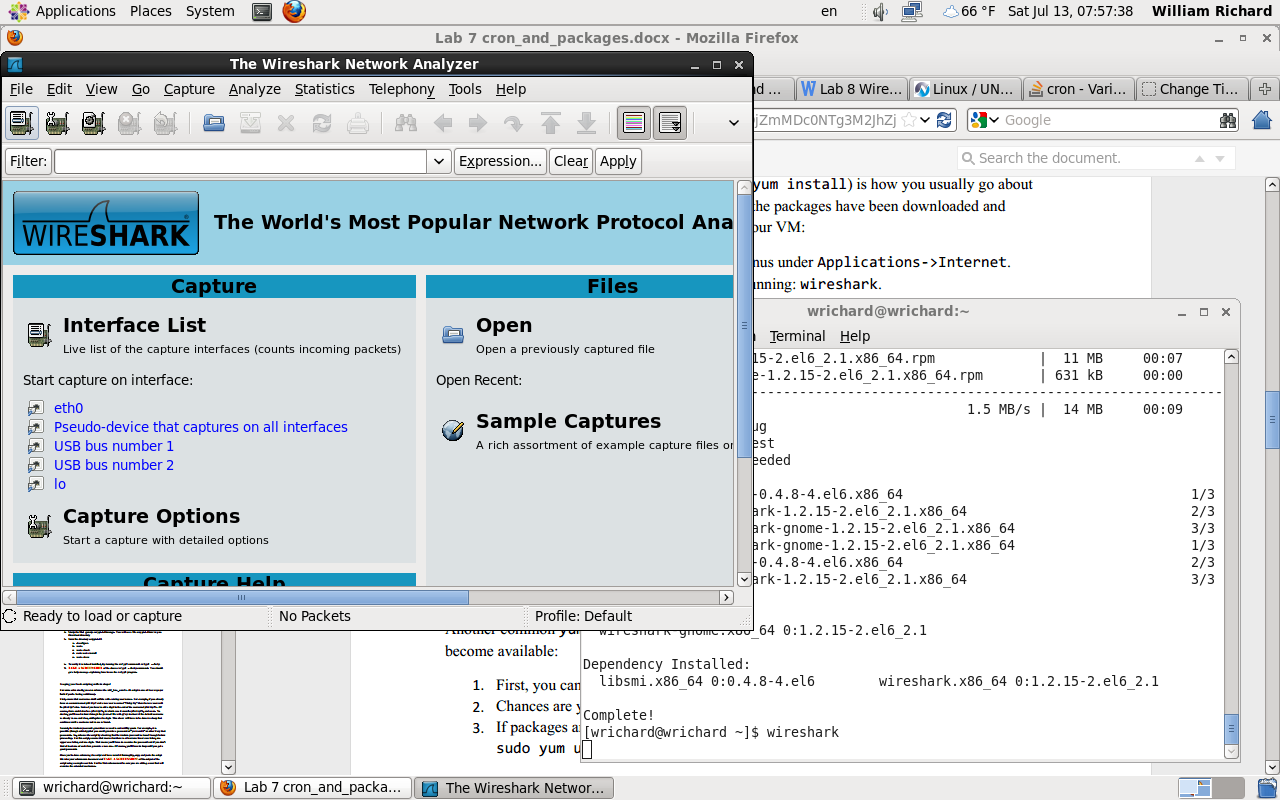
\includegraphics[width=\linewidth]{./datelog.png}
  \end{center}

\section{Packages}
\subsection{Wireshark}
  \begin{center}
  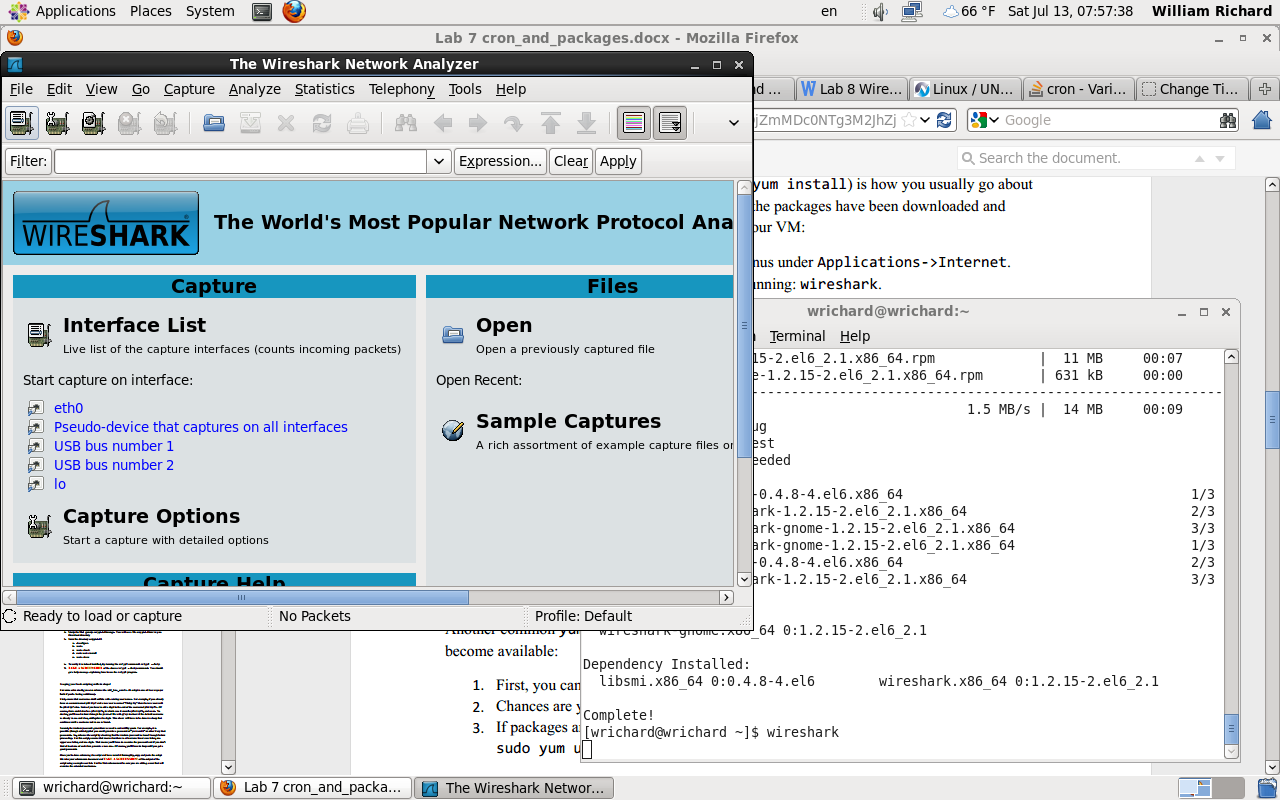
\includegraphics[width=\linewidth]{./wireshark.png}
  \end{center}
\subsection{ccrypt}
  \begin{center}
  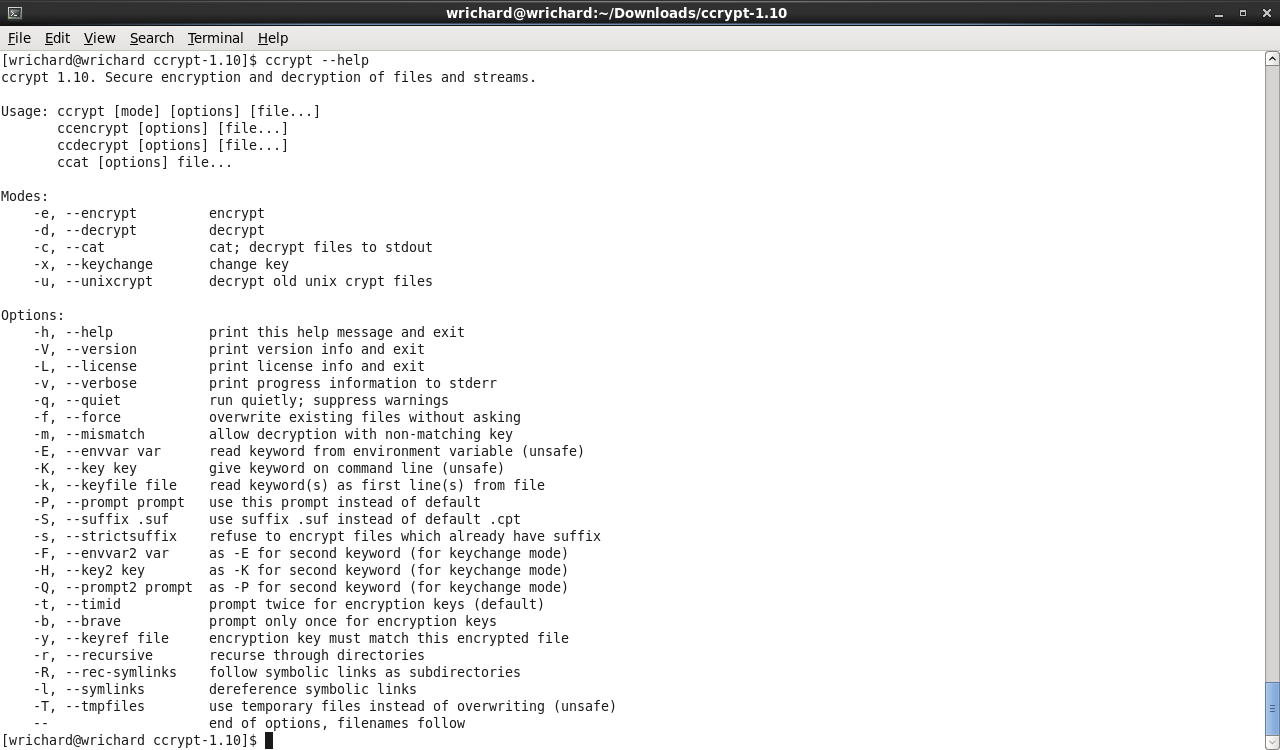
\includegraphics[width=\linewidth]{./ccrypt.png}
  \end{center}


\end{document}
